
\section{Architecture Overview}

DisJ simulation has been developed as Eclipse Plug-in application in which the simulation takes advantage of reusing many existing applications in Eclipse platform. The Eclipse is an extendable platform that provides useful building blocks and frameworks that facilitate developing new seamlessly-integrated applications. These frameworks and building blocks are exposed via well-defined API interfaces, classes, and methods that become mechanisms to use and rules to follow. Plug-in is a smallest unit of Eclipse Platform that can be developed, it consists of Java code Java Archive library, some read-only files, and other resources such as images, web templates, message catalogs, native code libraries etc like any normal Java applications.

There are many plug-ins that DisJ uses and requires e.g. Core plug-ins provides many foundation components that required by the simulation such as runtime management, file system, network, data binding, resource management etc, Java Development Tool (JDT) provides IDE for Java code editor that assists, validate and compile Java codes etc, Graphical Editor Framework (GEF) provides 2D graphical drawing tools that used by graph editor to display and edit graph topology. A hight level architecture has been shown in Figure~{\ref{pic:fig40}}.

\begin{figure}[ht!]
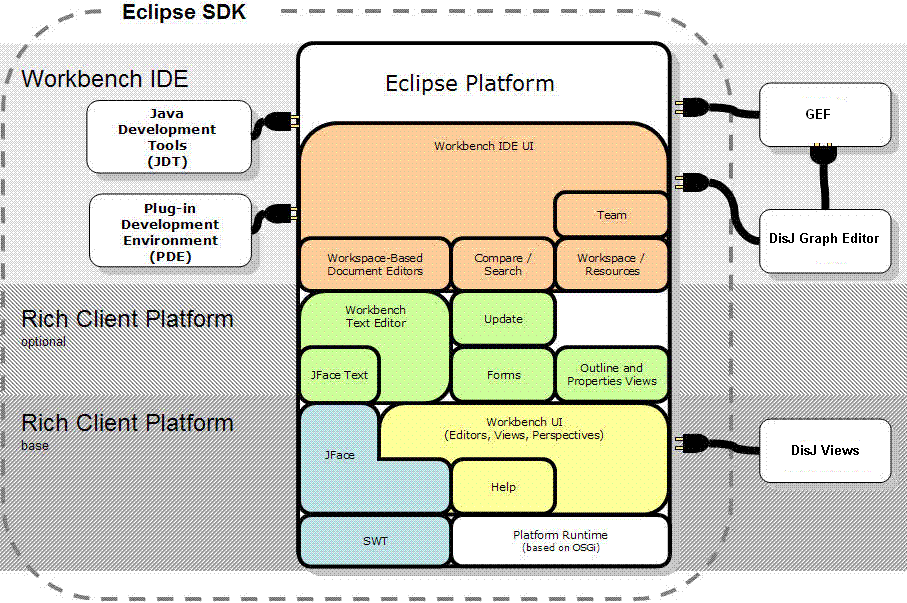
\includegraphics[width=1.0\textwidth,keepaspectratio]{./figure40}
\caption{DisJ Simulation Plug-in with Eclipse}
\label{pic:fig40}
\end{figure}


\section{Architecture and Design}

The simulation has been designed with multiple components, in which it helps to reduce the complexity of the system into small components with less complexity and easier to develop and maintenance. There are four main components as shown in Figure~{\ref{pic:fig41}}.

\begin{figure}[ht!]
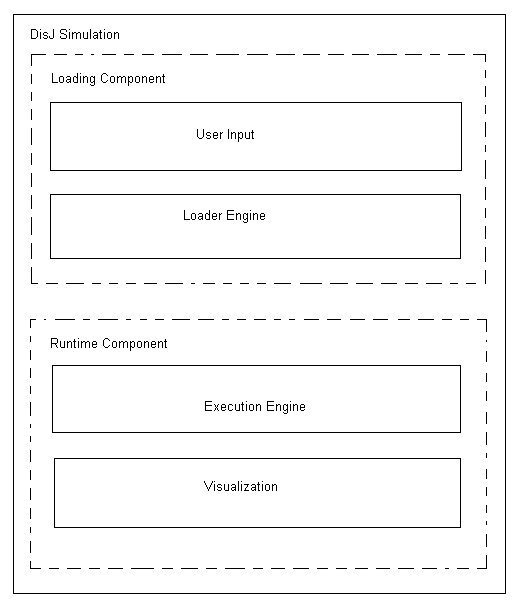
\includegraphics[width=1.0\textwidth,keepaspectratio]{./figure41}
\caption{DisJ Simulation High Level View}
\label{pic:fig41}
\end{figure}


\subsection{Loading Environment}

Loading environment is an environment for preparing and setting data that are needed for the simulation to execute. Components in the environment are responsible to make sure that every data and information that needs to be executed are created and loaded into the environment before the execution process begins. Also within this environment all data that are needed during runtime must be loaded before the execution process starts. The environment is composed of two components as shown in Figure~{\ref{pic:fig42}}.

\begin{figure}[ht!]
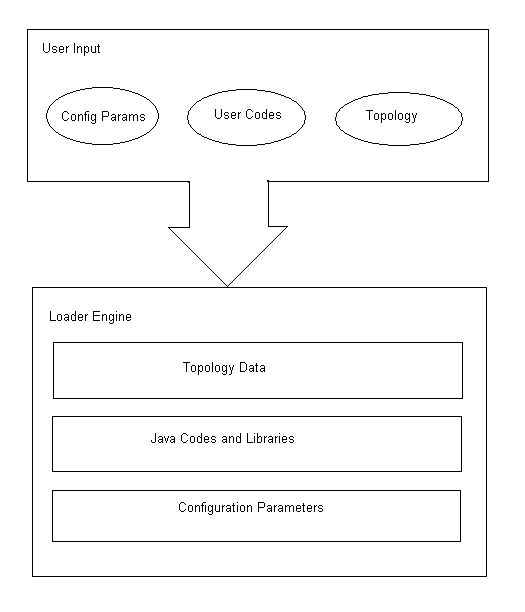
\includegraphics[width=1.0\textwidth,keepaspectratio]{./figure42}
\caption{Loading Environment}
\label{pic:fig42}
\end{figure}

\begin{enumerate}
\item{User Input}
This component is an interface between the simulation and user, in which it will extract and validate user algorithm and corresponding topology into the environment. The following will discuss some detail about subcomponents of User Input.

\begin{enumerate}
\item{Java Editor} is a component that allows user to provide an algorithm in Java programming language. The editor provides Java Development Tool (JDT) to help user in coding Java program like any other Java IDE.

\item{Graph Editor} is a Graphical User Interface (GUI) editor panel that provides a tool for user to specify topology and it properties that the algorithm will run through it as a sample network environment. The editor also allows user to load from or save to a file system as persistence storage in order to reuse a same topology in difference occasion.
\end{enumerate}

\item{Loading Engine}
Loading engine is a component that responsible for loading data from User Input and other necessary data into a working space of the simulation before hand over to Runtime Environment. A working space is created by loading engine, in one to one mapping to an execution of the simulation, and used by runtime environment. The working space contains many important data such as topology data, API libraries, and configuration parameters.

\begin{enumerate}
\item{Topology Data} is a data structure that contains all necessary information about the topology created in Graph Editor, in which any change of data by the simulation will affect the display in Graph Editor.

\item{API Libraries} is a set of all API used by the simulation and user algorithm such as communication API, external plug-in libraries, and adversary program.

\item{Configuration Parameters} that related to the execution of the simulation configured by user before the start of the simulation such as network environment, number of agents, number of token etc. These configuration parameters are data that must be provided before the starting of the simulation and cannot be modified once the simulation started.
\end{enumerate}
\end{enumerate}


\subsection{Runtime Environment}
Runtime environment is an environment that contains components that requires by the simulation during the execution of the simulation such as Execution Engine, Virtual Animation and Adversary Interruption.


\subsection{Execution Engine}
The execution engine is a core engine that drives and manages the execution of the simulation. The execution engine will create an execution process in one to one mapping to a work space that has been created during loading environment. The execution process virtually contains five components that processes user algorithm by using a discrete event processing technique to simulation the execution.

\begin{figure}[ht!]
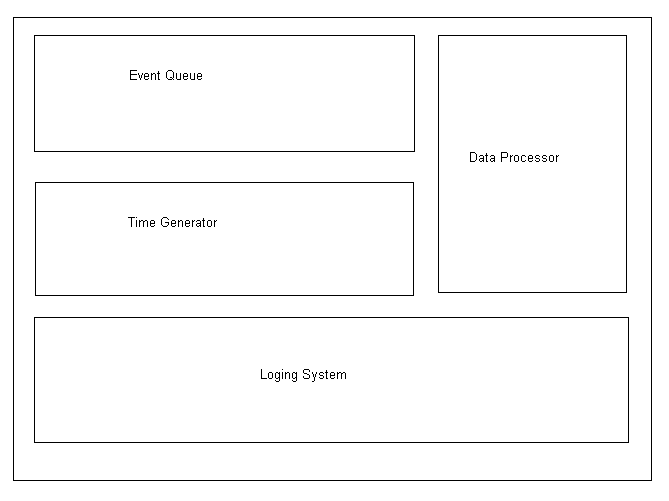
\includegraphics[width=1.0\textwidth,keepaspectratio]{./figure43}
\caption{Execution Engine}
\label{pic:fig43}
\end{figure}


\begin{enumerate}
\item{Event Queue}
An event is a collection of data set, which contains necessary data about the execution and a timestamp to execute this event.

\item{Event Queue}
An event queue is an ordered queue of events by timestamp. The queue provide a sequence of executed events based on the time that event will be occurred. Any time that a new event arrive the queue will insert the event into an appropriated position based on the timestamp assigned to the event. However, the timestamp will never be smaller than a timestamp of a top event in a queue, in which the time generator will take care of.

\item{Time Generator}
Timestamp is a time defined by the simulation, called a simulation time unit, the time of the simulation will always be increasing order from the starting of the simulation to the end. A time generator is an engine that will generate a timestamp of each event created by Data Processor. The time generator will assign a new timestamp to a new event based on a current simulation time and condition parameters provided by the data process in which the new time will be equal or bigger than a current.

\item{Data Processor}
Data processor is an engine that executes an event when a timestamp is equal to a simulation time. Each execution may or may not proceed to a creation of new event or events, which entirely based on the data contains in the event, the simulation configuration parameters and adversary interruption program. Any new event created will be assigned a timestamp of execution and inserted into an event queue. In addition, the execution of event may lead to a change of states of user algorithm and visual animation which discuss in later section.

\item{Logger}
A logger is a unit that logging events occurred during the execution of the simulation. Information that is logged will be used for replay of the simulation and debugging purposes.
\end{enumerate}


\subsection{Visualization}
The visualization of the simulation can be categorized into two separate parts, Editor part and View part.

\subsubsection{Editor Part}
DisJ graph editor is a main playground for user to create and modify graph and topology for the simulation to simulate an algorithm. The editor is an extension of GEF graphical editor that provides many tools for 2D graphical drawing. The editor consists of three parts

\begin{figure}[ht!]
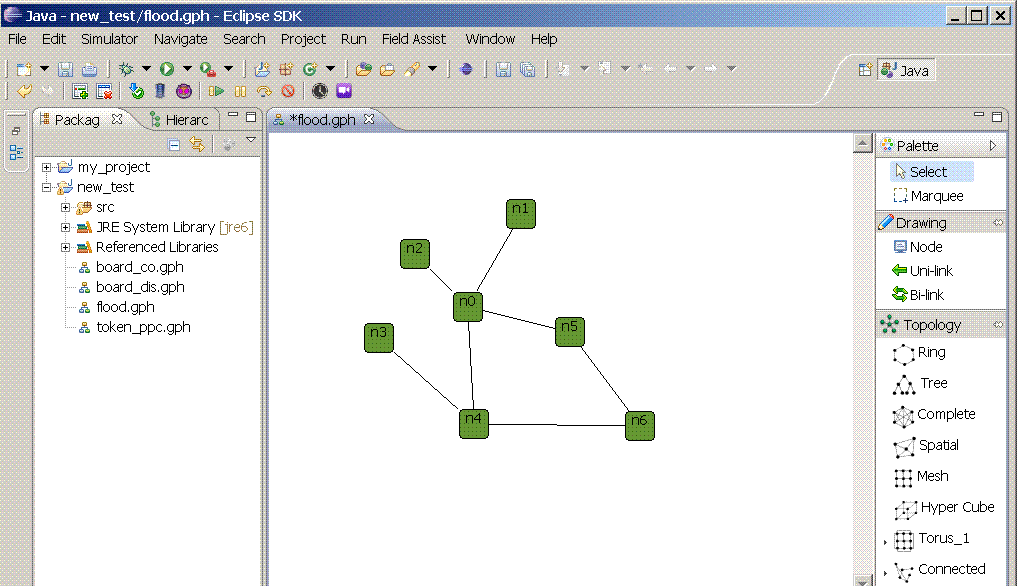
\includegraphics[width=1.0\textwidth,keepaspectratio]{./figure44}
\caption{DisJ Simulation: Graph Editor}
\label{pic:fig44}
\end{figure}


\begin{enumerate}
\item A drawing canvas that allows user to draw a 2D graphical of nodes and links
\item A Palette is a container that contains tools and figures for drawing objects
\item A Menu bar for user to issue commands to the simulation
\end{enumerate}

\subsubsection{View Part}
Eclipse platform provides a view extension that allows the simulation to create multiple views to display difference objects and perspectives of the simulation. DisJ simulation currently provides six separate views that display difference type of information to user as follow

\begin{figure}[ht!]
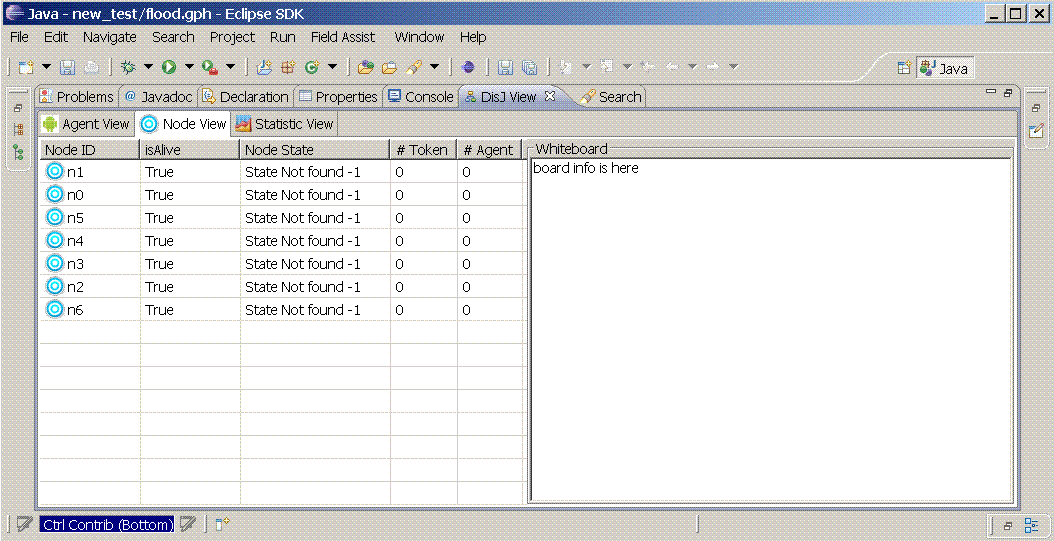
\includegraphics[width=1.0\textwidth,keepaspectratio]{./figure45}
\caption{DisJ Simulation: Node View}
\label{pic:fig45}
\end{figure}

\begin{enumerate}
\item An overview view that capture overall canvas into a readonly view that fit into a screen
\item A properties view is a view that display properties of a selected object in graph editor canvas
\item Node view is a view that display every nodes current information in real time
\item Agent view is a view that display every agent current information in real time
\item Console view is a view that display system and information texts provided by the simulation
\item Statistic view is a view that display statistical bar chart information of an algorithm execution in real time
\end{enumerate}


\subsection{Playback and Replay}
Playback is a series of display changed in DisJ simulation while the simulation is executing. The display is changed based on the change of entities states and information during the execution of an algorithm. The simulation does record states and information changes during the execution of algorithm into persistence storage, file I/O, in order for DisJ replay system to read and replay the execution in later time. The records are stored in a plain text with curtain predefined formate of text structure in order for the replay system can read and parse the data and execute the replay correctly.

\begin{figure}[ht!]
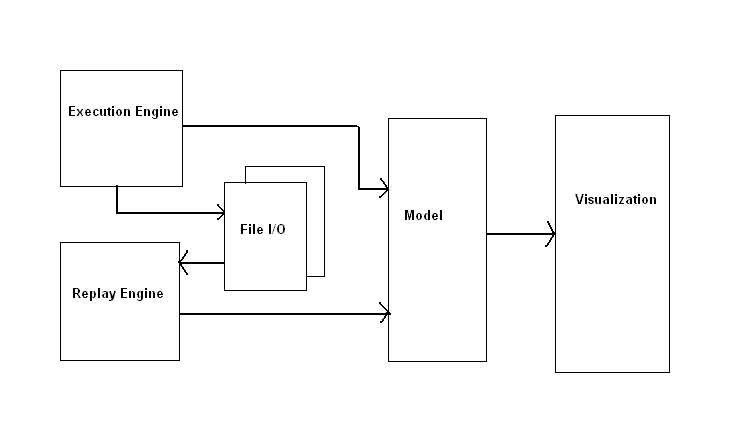
\includegraphics[width=1.0\textwidth,keepaspectratio]{./figure46}
\caption{Playback and Replay Architecture}
\label{pic:fig46}
\end{figure}


\subsection{Adversary Interruption}

The adversary interruption is a module that DisJ simulation allows user to plug-in an adversary program into the simulation in order to verify and test correctness of an algorithm during an execution runtime. The simulation provide interface for the adversary program to access information and control certain parts of the system in order to control and direct environment and its behavior for testing and verifying the correctness and response of the algorithm. However, it is user responsible to make sure that adversary code does not break certain rules and definitions of the environment, since adversary code has control of environment behaviors.

The simulation provides an abstract class for user to extends and the simulation provides API for adversary to access environment information and control its behaviors. The abstract class has some functions that you can implements functionalities in order to control behaviors of environment, in which the simulation will execute those functions, if it has been implemented, instead of default implementation of the system.

// figure 7 Add figure of work flow how adv scripts effect and done in the system


The simulation has an execution engine as an interface to interact with adversary interruption API in order to check and validate the decision based on user implemented adversary codes. The user adversary program is more likely mapping one to one to an algorithm and a topology given for an execution due to the environment control that has been coded in the adversary program which may specifically specify certain parameters and conditions of the environment to act at certain ways.


\subsection{Probability Model Extension}
Probability Model Extension is a module that DisJ simulation provide an option for user to plug-in customs or existing probability model into the simulation. Since, the simulation provides only two probability model, Uniform Random and Poisson Random, in which they are basic and general probability model. By default the simulation use Uniform Random model in controlling and making decision of environment.

The simulation provide an interface class for user to implement and the simulation always execute interface functions within the class when the probability is required during the simulation execution. Therefore, user can connect an external library via this interface class and the simulation engine will redirect the function calls to the library instead of default codes. This design works even the library is not in Java language, as long as user code in the implemented class able to interface and redirect a call to the external library. For example, the external library is in C/C++, user has two options, one is using JNI to redirect function calls or using socket communication from implemented class to the interface of the library.

// Add figure of work flow how prob model works with user lib


